\documentclass[12pt]{article}

\usepackage[utf8]{inputenc}
\usepackage[T1]{fontenc}
\usepackage{mathpazo}
\usepackage[margin=2.5cm]{geometry}
\usepackage{enumitem}
\usepackage{titlesec}
\usepackage{hyperref}
\usepackage{xcolor}
\usepackage{graphicx}

% Section formatting — small caps, no numbering
\titleformat{\section}{\normalsize\bfseries\scshape}{}{0em}{}
\titlespacing{\section}{0pt}{1.2em}{0.4em}

% No page numbers
\pagestyle{empty}

% Hyperlink style
\hypersetup{colorlinks=true, linkcolor=black, urlcolor=blue!60!black, citecolor=black}

\begin{document}

\begin{center}
{\Large\bfseries Virtual Qualia and the Dissolution of the Hard Problem:\\[0.15cm]
A Simulation-Based Framework 30 Years After \textit{The Conscious Mind}}

\vspace{0.6cm}

{\large Matthias Gruber}\\[0.15cm]
Independent Researcher\\[0.1cm]
\href{mailto:matthias@matthiasgruber.com}{matthias@matthiasgruber.com} \quad|\quad ORCID: \href{https://orcid.org/0009-0005-9697-1665}{0009-0005-9697-1665}
\end{center}

\vspace{0.3cm}
\noindent\rule{\textwidth}{0.4pt}
\vspace{0.3cm}

\noindent Chalmers (1996) established the Hard Problem as the central challenge for any theory of consciousness: why does physical processing give rise to subjective experience? Thirty years later, the field remains in a pre-paradigm state. The COGITATE adversarial collaboration found neither IIT nor GNW fully confirmed (COGITATE Consortium, 2025), and no existing framework simultaneously addresses the Hard Problem, the Explanatory Gap, binding, the boundary problem, and the structure of experience. This poster presents the Four-Model Theory (FMT; Gruber, 2015, 2026), which dissolves the Hard Problem by identifying a category error in its formulation---and derives testable consequences across psychopharmacology, sleep science, and clinical neurology.

\section{The Framework}

FMT proposes that consciousness consists of real-time self-simulation organized along two orthogonal dimensions---scope (world vs.\ self) and mode (implicit vs.\ explicit)---yielding four kinds of model as a principled minimum:

\begin{itemize}[nosep, leftmargin=1.5em]
\item \textbf{Implicit World Model (IWM):} substrate-level world knowledge (synaptic weights, learned regularities). Non-conscious.
\item \textbf{Implicit Self Model (ISM):} substrate-level self-knowledge (body schema, habits, autobiographical structures). Non-conscious.
\item \textbf{Explicit World Model (EWM):} the real-time simulation of reality---perceptual experience. Conscious.
\item \textbf{Explicit Self Model (ESM):} the real-time simulation of ``I''---self-experience. Conscious.
\end{itemize}

\begin{figure}[h]
\centering
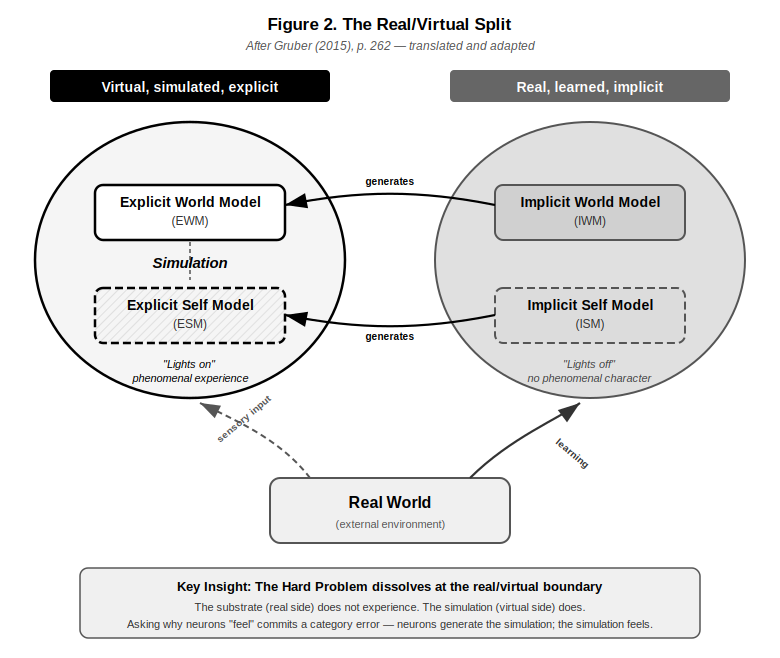
\includegraphics[width=0.78\textwidth]{../figures/figure2-real-virtual-split-bw.png}
\caption{The Real/Virtual Split. The implicit (real) side generates the explicit (virtual) side --- the simulation. The Hard Problem dissolves at this boundary: the substrate does not experience; the simulation does.}
\label{fig:architecture}
\end{figure}

\noindent The implicit models constitute the ``real side'' (structural, learned, lights-off); the explicit models constitute the ``virtual side'' (simulated, transient, lights-on). This is a functional taxonomy of model kinds, not a claim about discrete brain modules---the biological substrate implements an effectively uncountable number of overlapping models organized around these two axes.

\section{Dissolving the Hard Problem}

The central claim is that qualia are \emph{virtual}: they are how the simulated self (ESM) perceives its own states within the simulation. The physical substrate does not ``feel''---the simulation does, and within the simulation, qualia are constitutive. Asking why neuronal firing feels like something commits a category error analogous to asking why transistor switching feels like running a video game. The two-level ontology (substrate: no experience; simulation: genuine experience) closes the Explanatory Gap simultaneously: the gap between ``neurons fire in pattern X'' and ``I experience red'' reflects the level distinction, not a gap in knowledge.

This is not illusionism: qualia are real within the simulation. Nor is it dualism: both levels are physical. What dissolves is the assumption that phenomenal properties must be found at the substrate level.

Self-referential closure explains why this simulation, unlike a weather model, has experience: the ESM models the system's own modeling process, collapsing the distinction between model and modeled. A non-self-referential simulation has an outside from which it can be described without remainder; a self-referential simulation at criticality does not.

\section{Criticality and Convergence}

FMT requires the substrate to operate at the edge of chaos (Wolfram's Class~4 regime). This requirement, derived from computational first principles in 2015, converges with the empirical criticality program consolidated independently a decade later (Hengen \& Shew, 2025; Algom \& Shriki, 2026)---an instance of theoretical prediction preceding empirical confirmation.

\section{Novel Predictions}

The framework generates nine testable predictions, including: (1)~psychedelic ego dissolution content tracks dominant sensory input (the ESM, deprived of self-referential input, latches onto whatever input dominates); (2)~psychedelics at sub-ego-dissolution doses should alleviate anosognosia (global permeability increase overwhelms local permeability block); (3)~all anesthetics converge on criticality disruption regardless of receptor mechanism; (4)~sleep architecture reflects criticality maintenance (NREM/REM cycling tracks substrate oscillation around the critical point). Predictions (1) and (2) are cross-domain surprises that few competing theories generate.

\section{Significance for Chalmers' Program}

FMT engages directly with the problems Chalmers identified: it addresses the Hard Problem through virtual qualia and two-level ontology; it grounds the structure of experience in the simulation's generative architecture; it solves binding through the unity of the virtual world; it explains the Meta-Problem as an artifact of triply recursive self-modeling. The theory is offered not as a final answer but as a framework that takes Chalmers' challenge seriously enough to provide a dissolution rather than a deflection---and stakes its credibility on novel empirical predictions.

\vspace{0.5cm}
\noindent\rule{\textwidth}{0.4pt}
\vspace{0.2cm}

\noindent\textbf{References:} Gruber, M. (2015). \textit{Die Emergenz des Bewusstseins}. Self-published. ISBN 9781326652074. \,|\, Gruber, M. (2026). The Four-Model Theory of Consciousness. \textit{Zenodo} preprint. \href{https://doi.org/10.5281/zenodo.18669891}{doi:10.5281/zenodo.18669891}

\end{document}
